\section{Conexión y Compacidad}\label{sec:Rel3}

\begin{ejercicio}
Demuestra que $ \bb{S}^1 $ no es homeomorfo a ningún subconjunto de $ \bb{R} $ ambos considerados con la topología usual.\\


    Sea $A\subset \bb{R}$, y supongamos que $A$ es homeomorfo a $\bb{S}^1$, por lo que existe un homeomorfismo $f:\bb{S}^1 \to A$.
    Como $\bb{S}^1$ sabemos que es conexo, entonces $A$ también lo es, y como $A\subset \bb{R}$, entonces $A$ es un intervalo, supongamos de extremos
    $a$ y $b$, $a<b$, $a,b\in \bb{R}$, o $\pm \infty$.

    Sea ahora $c\in A$ tal que $a<c<b$, y como $f$ es biyectiva, consideremos su preimagen $f^{-1}(c)\in \bb{S}^1$.
    Sea entonces la restricción de $f$ a $\bb{S}^1\setminus \{f^{-1}(c)\}$,
    que es un homeomorfismo entre $\bb{S}^1\setminus \{f^{-1}(c)\}$ y $A\setminus \{c\}$. Como la esfera sin un punto es homeomorfa a $\bb{R}$ (conexo),
    entonces es $A\setminus \{c\}\subset \cc{R}$ es conexo, por lo que es un intervalo. No obstante, esto es una contraddicción,
    ya que $A\setminus \{c\}$ no es un intervalo por tener $a,b\in A\setminus \{c\}$ y $c\notin A\setminus \{c\}$.

\end{ejercicio}

\begin{ejercicio}
Demuestra que $ A=\bb{R}^{n+1} \setminus \bb{S}^n $ no es conexo.\\

    Sea $U=\bb{R}^{n+1}\setminus \ol{B}(0,1)$, $V=B(0,1)$. Tenemos que $U,V\in \T_u$ abiertos de la topología usual de $\bb{R}^{n+1}$.
    Además, $U\cap A=U$ y $V\cap A=V$, por lo que $U,V\in \T_A$ abiertos en la topología usual inducida en $A$. Además, tenemos que $U,V\neq A,\emptyset$.

    Tenemos que $U\cap V=\left(\bb{R}^{n+1}\setminus \ol{B}(0,1)\right) \cap B(0,1)=\emptyset$, y:
    \begin{equation*}
        U\cup V
        = \left(\bb{R}^{n+1}\setminus \ol{B}(0,1)\right) \cup B(0,1)
        = \bb{R}^{n+1} \setminus \bb{S}^n
        = A
    \end{equation*}
    Por tanto, $A$ es conexo.

\end{ejercicio}

\begin{ejercicio}
    Sea $(X, \T)$ un espacio topológico. Demuestra que son equivalentes:
    \begin{enumerate}
        \item $(X, \T)$ es conexo.
        \item Para todo $A \subseteq X$ tal que $\partial A = \emptyset$ se tiene $A = X$ o $A = \emptyset$.
    \end{enumerate}

    Veamos en primer que lugar que, dado $A\subset X$, se tiene que $\partial A=\emptyset$ si y solo si $A$ es abierto y cerrado.
    \begin{description}
        \item[$\Longrightarrow)$]  Supongamos que $\partial A=\emptyset$. Entonces,
        \begin{equation*}
            \emptyset = \partial A = \ol{A} \setminus A^\circ \Longleftrightarrow \ol{A} \subset A^\circ
        \end{equation*}
        Como $A^\circ \subset A\subset \ol{A}$, entonces $A^\circ = \ol{A} = A$, por lo que $A$ es cerrado y abierto.

        \item[$\Longleftarrow)$] Supongamos que $A$ es abierto y cerrado. Entonces,
        \begin{equation*}
            \partial A = \ol{A} \setminus A^\circ = A \setminus A = \emptyset
        \end{equation*}
        Por tanto, $\partial A=\emptyset$.
    \end{description}

    Tenemos por tanto las siguientes equivalencias:
    \begin{enumerate}
        \item $(X, \T)$ es conexo.
        \item Para todo $A \subseteq X$ tal que $A$ es abierto y cerrado se tiene $A = X$ o $A = \emptyset$.
        \item Para todo $A \subseteq X$ tal que $\partial A = \emptyset$ se tiene $A = X$ o $A = \emptyset$.
    \end{enumerate}
    La equivalencia entre 1) y 2) se ha demostrado en la Caracterización de la Conexión, y la equivalencia entre 2) y 3) se ha demostrado en este ejercicio.
\end{ejercicio}

\begin{ejercicio}
    Sean $A$ y $B$ subconjuntos conexos de un espacio topológico $(X, \T)$ tales que $\ol{A} \cap B = \emptyset$. Demuestra que $A \cup B$ es conexo.\\

    Como $\ol{A}\cap B\neq \emptyset$, entonces $\exists b_0\in \ol{A}\cap B$. Como $A$ es conexo y $A\subset A\cup \{b_0\}\subset \ol{A}$, por el Teorema \ref{teo:AdherenciaConexo}
    tenemos que $A\cup \{b_0\}$ es conexo.

    Tenemos que $A\cup B = \left(A\cup \{b_0\}\right)\cup B$, siendo ambos conexos. Además, como se tiene que $b_0\in \left(A\cup \{b_0\}\right)\cap B\neq \emptyset$, por el Teorema \ref{prop:UnionConexos}, $A\cup B$ es conexo.
\end{ejercicio}

\begin{ejercicio}
    Sean $A$ y $B$ subconjuntos cerrados y no vacíos de un espacio $(X, \T)$ tales que $A \cup B$ y $A \cap B$ son conexos. Demuestra que $A$ y $B$ son conexos.\\

    Supongamos que $A$ no es conexo, por lo que existen $C,D\in C_{\T_A}$ cerrados de $A$ no triviales tales que $C\cap D = \emptyset$ y $C\cup D = A$.
    Por ser cerrados de $A$, existen $C',D'\in C_{\T}$ tales que $C=C'\cap A$ y $D=D'\cap A$,
    y como $A\in C_{\T}$ y la intersección de cerrados en cerrado, tenemos que $C,D\in C_\T$.

    Consideramos ahora $A\cap B\subset A=C\cap D$. Veamos ahora que $A\cap B$ solo interseca a uno de los dos conjuntos $C$ y $D$.
    Por contrarecíproco, supongamos $(A\cap B)\cap C\neq \emptyset$ y $(A\cap B)\cap D\neq \emptyset$. Entonces, sean $\wt{C}=(A\cap B)\cap C$ y $\wt{D}=(A\cap B)\cap D$, ambos no vacíos.
    Tenemos que $\wt{C},\wt{D}\in C_{\T_{A\cap B}}$. Además:
    \begin{gather*}
        \wt{C}\cap \wt{D}
        = [(A\cap B)\cap C] \cap [(A\cap B)\cap D] \subset C\cap D = \emptyset \\
        \wt{C}\cup \wt{D}
        = [(A\cap B)\cap C] \cup [(A\cap B)\cap D]
        = (A\cap B)\cap (C\cup D) = (A\cap B)\cap A = A\cap B
    \end{gather*}
    Por tanto, tenemos que $\wt{C},\wt{D}\in C_{\T_{A\cap B}}$ cerrados de $A\cap B$ no triviales tales que $\wt{C}\cap \wt{D}=\emptyset$ y $\wt{C}\cup \wt{D}=A\cap B$,
    por lo que $A\cap B$ no es conexo, lo que es una contradicción.

    Por tanto, $A\cap B\subset C$ o $A\cap B\subset D$.
    Supongamos sin pérdida de generalidad que $A\cap B\subset C$.
    Entonces, $A\cap B\subset C$, y como $C\cap D=\emptyset$, entonces $(A\cap B)\cap D = \emptyset$. Como $D\subset A$, entonces $B\cap D=\emptyset$. Entonces:
    \begin{gather*}
        A\cup B = (C\cup D)\cup B = D \cup (C\cup B)\\
        D\cap (C\cup B) = (D\cap C) \cup (D\cap B) = \emptyset \cup \emptyset = \emptyset
    \end{gather*}
    Como $D$ es no trivial, entonces $C\cup B$ es no trivial. Además, como $C,D,B\subset A\cup B$ y los tres son cerrados, tenemos que $D,C,B\in C_{\T_{A\cup B}}$.
    Como la unión finita de cerrados es cerrado, entonces $C\cup B\in C_{\T_{A\cup B}}$. Por tanto, tenemos una partición de $A\cup B$ en dos cerrados no triviales,
    por lo que $A\cup B$ no es conexo, lo que es una contradicción.
    
    Por tanto, $A$ es conexo. Intercambiando $A$ por $B$, se demuestra que $B$ es conexo.
\end{ejercicio}

\begin{ejercicio} \label{ej:Rel3.6}
    Sean $Y_1$ y $Y_2$ subespacios de $(X, \T)$ y sea $A \subseteq Y_1 \cap Y_2$.
    Demuestra que si $A$ es abierto (respectivamente cerrado) en $Y_1$ y en $Y_2$, entonces $A$ es abierto (respectivamente cerrado) en $Y_1 \cap Y_2$ y en $Y_1 \cup Y_2$.\\

    Como $A\in \T_{Y_1}$, tenemos que $\exists A_1\in \T$ tal que $A=A_1\cap Y_1$. Análogamente, $\exists A_2\in \T$ tal que $A=A_2\cap Y_2$. Notemos que $A_1\cup A_2, A_1\cap A_2\in \T$.

    Como $A_1\cup A_2\in \T$, tenemos que $(A_1\cup A_2)\cap (Y_1\cap Y_2)\in \T_{Y_1\cap Y_2}$. Además,
    \begin{align*}
        (A_1\cup A_2)\cap (Y_1\cap Y_2) &= (A_1\cap Y_1 \cap Y_2)\cup (A_2\cap Y_1\cap Y_2) =\\&= (A\cap Y_2) \cup (A\cap Y_1) = A \cap (Y_1\cup Y_2) = A
    \end{align*}
    Por tanto, $A\in \T_{Y_1\cap Y_2}$. Además, como $A_1\cap A_2\in \T$, tenemos que $(A_1\cap A_2)\cap (Y_1\cup Y_2)\in \T_{Y_1\cup Y_2}$. Además,
    \begin{align*}
        (A_1\cap A_2)\cap (Y_1\cup Y_2) &= (A_1\cap A_2 \cap Y_1)\cup (A_1\cap A_2 \cap Y_2) =\\&= (A\cap A_2) \cup (A\cap A_1) = A \cap (A_1\cup A_2) = A
    \end{align*}
    donde he empleado que $A \subset A_1,A_2$, por lo que $A\subset A_1\cup A_2$. Por tanto, $A\in \T_{Y_1\cup Y_2}$.

    Por tanto, hemos visto que $A\in \T_{Y_1\cap Y_2}$ y $A\in \T_{Y_1\cup Y_2}$, por lo que $A$ es abierto en $Y_1\cap Y_2$ y en $Y_1\cup Y_2$. La demostración para cerrados es análoga,
    ya que la intersección y la unión de dos cerrados es cerrado.
\end{ejercicio}

\begin{ejercicio}
    Sean $(X, \T)$ un espacio conexo y $A$ un subconjunto conexo y no vacío de $X$. Sea $U$ un abierto y cerrado en $X \setminus A$. Demuestra que $A \cup U$ es conexo.

    Supongamos que es disconexo, por lo que existe $V\in \T_{A\cup U}\cap C_{\T_{A\cup U}}$ abierto y cerrado de $A\cup U$ no trivial ($V\neq \emptyset,~V\neq A\cup U$).
    Como $V\in \T_{A\cup U}$, entonces $\exists V'\in \T$ tal que $V=V'\cap (A\cup U)$. Por tanto, $A\cap V = A\cap V'\cap (A\cup U) = A\cap V'$, por lo que $A\cap V\in \T_A$.
    Análogamente, se ve que $A\cap V\in C_{\T_A}$, por lo que $A\cap V$ es abierto y cerrado de $A$ no trivial. Como $A$ es conexo, entonces $A\cap V$ es trivial, por lo que $A\cap V=\emptyset$ o $A\cap V=A$.
    \begin{enumerate}
        \item Supongamos $A\cap V=\emptyset$.
        
        Como $U\subset X\setminus A$ y $V\subset A\cup U$, entonces $V\subset U$. Además, $U\cap V = U\cap V'$, por lo que $V=U\cap V\in \T_{U}$.
        Análogamente, $V\in C_{\T_{U}}$, por lo que $V\in \T_{U}\cap C_{\T_{U}}$. Como $U\in \T_{X\setminus A}\cap C_{\T_{X\setminus A}}$,
        entonces $V\in \T_{X\setminus A}\cap C_{\T_{X\setminus A}}$, por lo que $V$ es abierto y cerrado de $X\setminus A$.

        Aplicamos ahora el Ejercicio \ref{ej:Rel3.6} al conjunto $V$, con $Y_1=X\setminus A$, $Y_2=U\cup A$. Tenemos que $V\subset U\subset Y_1 \cap Y_2$, y
        $V\in \T_{Y_1}\cap C_{\T_{Y_1}}$ y $V\in \T_{Y_2}\cap C_{\T_{Y_2}}$. Por tanto, $V\in \T_{Y_1\cup Y_2}\cap C_{\T_{Y_1\cup Y_2}}$. Calculemos ahora $Y_1\cup Y_2$:
        \begin{equation*}
            Y_1\cup Y_2 = (X\setminus A) \cup (U\cup A) = X
        \end{equation*}
        
        Por tanto $V\in \T\cap C_{\T}$. Como $(X,\T)$ es conexo, entonces $V$ es trivial, por lo que $V=\emptyset$ o $V=X$.
        Como $\emptyset \neq A \subset X$ y $A\cap V=\emptyset$, entonces $V\neq X$, por lo que $V=\emptyset$, lo que es una contradicción.

        \item Supongamos $A\cap V=A$.
        
        Sea $C=(A\cup U)\setminus V\in \T_{A\cup U}\cap C_{\T_{A\cup U}}$. Por tanto, $A\cap C \in \T_A\cap C_{\T_A}$, por lo que $A\cap C$ es abierto y cerrado de $A$, y como $A$ es conexo, entonces $A\cap C$ es trivial.
        Veamos que $A\cap C\neq A$. Tenemos que:
        \begin{equation*}
            A \cap C = A\Longleftrightarrow A\subset C \Longleftrightarrow A\cap V \subset (A\cup U)\setminus V \Longleftrightarrow A\cap V = \emptyset
        \end{equation*}
        Que no es el caso, por lo que $A\cap C\neq A$. Por tanto, $A\cap C=\emptyset$. Aplicando el apartado anterior a $A\cap C$, tenemos que $C=\emptyset$, por lo que $A\cup U \subset V$. No obstante, sabemos que
        $V\subset A\cup U$, por lo que $A\cup U = V$, lo que es una contradicción.
    \end{enumerate}
\end{ejercicio}

\begin{ejercicio}
    Sean $(X, \T)$ un espacio conexo y $A$ un subconjunto conexo y no vacío de $X$. Sea $C$ una componente conexa de $X \setminus A$. Demuestra que $X \setminus C$ es conexo.\\

    Supongamos que $X\setminus C$ es disconexo, por lo que existe $U \in \T_{X\setminus C}\cap C_{\T_{X\setminus C}}$ abierto y cerrado de $X\setminus C$
    no trivial. Como $U\in \T_{X\setminus C}$, entonces $\exists U'\in \T$ tal que $U=U'\cap (X\setminus C)$. Por tanto, $A\cap U=A\cap (X\setminus C) \cap U' = A\cap U'$, donde he aplicado que,
    como $C\subset X\setminus A$, entonces $A\subset X\setminus C$. Por tanto, $A\cap U\in \T_A$. Análogamente, se ve que $A\cap U\in C_{\T_A}$, por lo que $A\cap U$ es abierto y cerrado de $A$. Como $A$ es conexo,
    entonces $A\cap U$ es trivial, por lo que $A\cap U=\emptyset$ o $A\cap U=A$.
    \begin{enumerate}
        \item Supongamos $A\cap U=A$. Entonces, $A\subset U$, y por tanto $A\cap X\setminus (U\cup C) = \emptyset$. Como $C\subset X\setminus A$ y $X\setminus (U\cup C)\subset X\setminus A$, entonces
        $C\subset C\cup X\setminus (U\cup C) \subset X\setminus A$, por lo que $A\cap \left(C\cup X\setminus (U\cup C)\right) = \emptyset$.

        \item Supongamos $A\cap U=\emptyset$. Entonces, $A\subset X\setminus U$, y como $A\subset X\setminus C$, entonces $A\subset X\setminus (U\cup C)$.
    \end{enumerate}
\end{ejercicio}

\begin{ejercicio}
    Prueba que el interior y la frontera de un subconjunto conexo no son en general conexos.\\

    Sea $(\bb{R}^2,\T_u)$ el espacio topológico. Sean $A=\ol{B}[(-1,0), 1], B=\ol{B}[(1,0), 1]\subset \bb{R}^2$ dos bolas cerradas. Estas son convexas, luego son conexos. Además, $A\cap B=\{(0,0)\}\neq \emptyset$, por lo que
    $A\cup B$ es conexo. Sin embargo, $[A\cup B]^\circ=B[(-1,0),1] \cup B[(1,0),1]$, que no es conexo por ser unión de dos abiertos disjuntos.

    Para el caso de la frontera, consideremos $A=[0,1]\times \bb{R}$. Tenemos que es conexo por ser producto de conexos.
    No obstante, $\partial A = (\{0\}\times \bb{R}) \cup (\{1\}\times \bb{R})$, que no es conexo por ser unión de dos cerrados disjuntos.


\end{ejercicio}

\begin{ejercicio}
    Sean $(X, \T)$ y $(X', \mathcal{T'})$ dos espacios topológicos conexos y $A \subsetneq X$, $B \subsetneq X'$. ¿Es $(X \times X') \setminus (A \times B)$ conexo?

    Para probar que sí es conexo, emplearemos la Proposición \ref{prop:PropiedadesComponentesConexas}, demostrando que
    tan solo tiene una componente conexa. Para ello, fijado $(a,b)\in (X\setminus A)\times (X'\setminus B)$, veremos que,
    para todo $(x,y)\in (X \times X') \setminus (A \times B)$, existe un conjunto conexo
    $D_{x,y}\subset (X \times X') \setminus (A \times B)$ con $(a,b),(x,y)\in D_{x,y}$.
    Como $D_{x,y}$ es conexo y $(a,b)\in D_{x,y}$, entonces $(x,y)\in D_{x,y}\subset C(a,b)$.
    Es decir, para todo $(x,y)\in (X \times X') \setminus (A \times B)$, se tiene que $(x,y)\in C(a,b)$, por lo que
    es la única componente conexa de $(X \times X') \setminus (A \times B)$, por lo que este conjunto es conexo.

    El siguiente dibujo ilustra la idea intuitiva del conjunto $D_{x,y}$:
    \begin{figure}[H]
        \centering
        \begin{subfigure}[c]{0.45\linewidth}
            \centering
            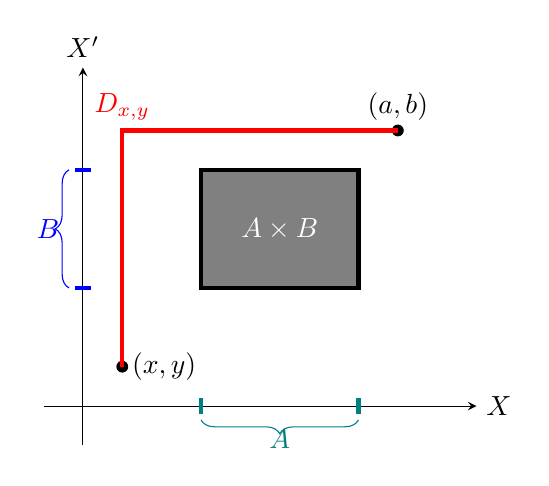
\begin{tikzpicture}
                \def\x{0.5}
                \def\y{0.5}
                \def\a{4}
                \def\b{3.5}
    
                % Ejes cartesianos
                \draw[-stealth] (-0.5, 0) -- (5, 0) node[right] {$X$};
                \draw[-stealth] (0, -0.5) -- (0, 4.3) node[above] {$X'$};
    
                % Marcas en el eje horizontal del conjunto A
                \draw[ultra thick, teal] (1.5,0.1) -- (1.5,-0.1);
                \draw[ultra thick, teal] (3.5,0.1) -- (3.5,-0.1);
                % Señalizacion A
                \draw[decorate,decoration={brace,amplitude=5pt,mirror}, teal, yshift=-5pt]
                (1.5,0) -- (3.5,0) node[midway,below] {$A$};
    
                % Marcas en el eje horizontal del conjunto B
                \draw[ultra thick, blue] (0.1,1.5) -- (-0.1,1.5);
                \draw[ultra thick, blue] (0.1,3) -- (-0.1,3);
                % Señalizacion B
                \draw[decorate,decoration={brace,amplitude=5pt}, blue, xshift=-5pt]
                (0,1.5) -- (0,3) node[midway,left] {$B$};
                
                % Conjunto AxB
                \draw[fill=gray, ultra thick] (1.5,1.5) rectangle (3.5,3);
                \node[white] at (2.5,2.25) {$A\times B$};
    
                % Punto (a,b)
                \fill (\a,\b) circle (0.075);
                \node[above] at (\a,\b) {$(a,b)$};
    
                % Punto (x,y)
                \fill (\x,\y) circle (0.075);
                \node[right] at (\x,\y) {$(x,y)$};
    
                % Conjunto D_{x,y}
                \draw[red, ultra thick] (\x,\y) -- (\x,\b) -- (\a,\b);
                \node[red, above] at (\x,\b) {$D_{x,y}$};
            \end{tikzpicture}
            \caption{$x\notin A, y\notin B$.}
            \label{fig:Rel3.11.a}
        \end{subfigure} \hfill
        \begin{subfigure}[c]{0.45\linewidth}
            \centering
            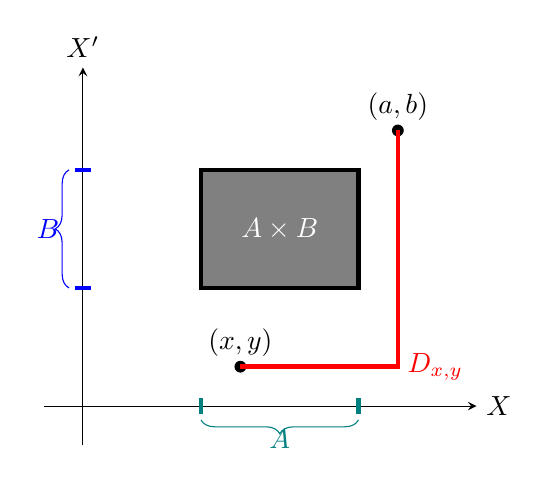
\begin{tikzpicture}
                \def\x{2}
                \def\y{0.5}
                \def\a{4}
                \def\b{3.5}
    
                % Ejes cartesianos
                \draw[-stealth] (-0.5, 0) -- (5, 0) node[right] {$X$};
                \draw[-stealth] (0, -0.5) -- (0, 4.3) node[above] {$X'$};
    
                % Marcas en el eje horizontal del conjunto A
                \draw[ultra thick, teal] (1.5,0.1) -- (1.5,-0.1);
                \draw[ultra thick, teal] (3.5,0.1) -- (3.5,-0.1);
                % Señalizacion A
                \draw[decorate,decoration={brace,amplitude=5pt,mirror}, teal, yshift=-5pt]
                (1.5,0) -- (3.5,0) node[midway,below] {$A$};
    
                % Marcas en el eje horizontal del conjunto B
                \draw[ultra thick, blue] (0.1,1.5) -- (-0.1,1.5);
                \draw[ultra thick, blue] (0.1,3) -- (-0.1,3);
                % Señalizacion B
                \draw[decorate,decoration={brace,amplitude=5pt}, blue, xshift=-5pt]
                (0,1.5) -- (0,3) node[midway,left] {$B$};
                
                % Conjunto AxB
                \draw[fill=gray, ultra thick] (1.5,1.5) rectangle (3.5,3);
                \node[white] at (2.5,2.25) {$A\times B$};
    
                % Punto (a,b)
                \fill (\a,\b) circle (0.075);
                \node[above] at (\a,\b) {$(a,b)$};
    
                % Punto (x,y)
                \fill (\x,\y) circle (0.075);
                \node[above] at (\x,\y) {$(x,y)$};
    
                % Conjunto D_{x,y}
                \draw[red, ultra thick] (\x,\y) -- (\a,\y) -- (\a,\b);
                \node[red, right] at (\a,\y) {$D_{x,y}$};
            \end{tikzpicture}
            \caption{$x\in A, y\notin B$.}
            \label{fig:Rel3.11.b}
        \end{subfigure}
        \begin{comment}
        \begin{subfigure}[c]{0.45\linewidth}
            \centering
            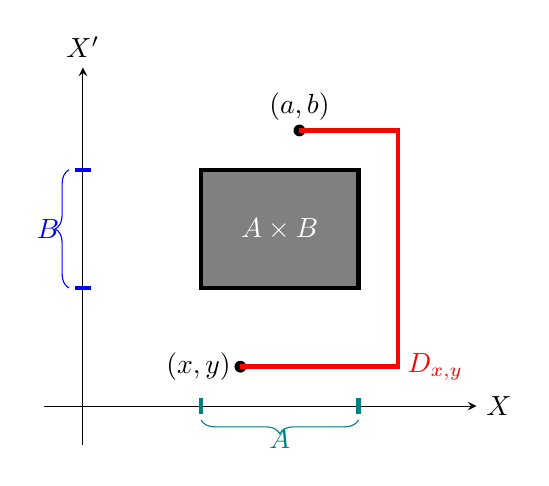
\begin{tikzpicture}
                \def\x{2}
                \def\y{0.5}
                \def\a{2.75}
                \def\b{3.5}
    
                % Ejes cartesianos
                \draw[-stealth] (-0.5, 0) -- (5, 0) node[right] {$X$};
                \draw[-stealth] (0, -0.5) -- (0, 4.3) node[above] {$X'$};
    
                % Marcas en el eje horizontal del conjunto A
                \draw[ultra thick, teal] (1.5,0.1) -- (1.5,-0.1);
                \draw[ultra thick, teal] (3.5,0.1) -- (3.5,-0.1);
                % Señalizacion A
                \draw[decorate,decoration={brace,amplitude=5pt,mirror}, teal, yshift=-5pt]
                (1.5,0) -- (3.5,0) node[midway,below] {$A$};
    
                % Marcas en el eje horizontal del conjunto B
                \draw[ultra thick, blue] (0.1,1.5) -- (-0.1,1.5);
                \draw[ultra thick, blue] (0.1,3) -- (-0.1,3);
                % Señalizacion B
                \draw[decorate,decoration={brace,amplitude=5pt}, blue, xshift=-5pt]
                (0,1.5) -- (0,3) node[midway,left] {$B$};
                
                % Conjunto AxB
                \draw[fill=gray, ultra thick] (1.5,1.5) rectangle (3.5,3);
                \node[white] at (2.5,2.25) {$A\times B$};
    
                % Punto (a,b)
                \fill (\a,\b) circle (0.075);
                \node[above] at (\a,\b) {$(a,b)$};
    
                % Punto (x,y)
                \fill (\x,\y) circle (0.075);
                \node[left] at (\x,\y) {$(x,y)$};
    
                % Conjunto D_{x,y}
                \draw[red, ultra thick] (\x,\y) -- (\x+2,\y) -- (\x+2,\b) -- (\a,\b);
                \node[red, right] at (\x+2,\y) {$D_{x,y}$};
            \end{tikzpicture}
            \caption{$x\in A, y\notin B$.}
        \end{subfigure}
        \begin{subfigure}[c]{0.45\linewidth}
            \centering
            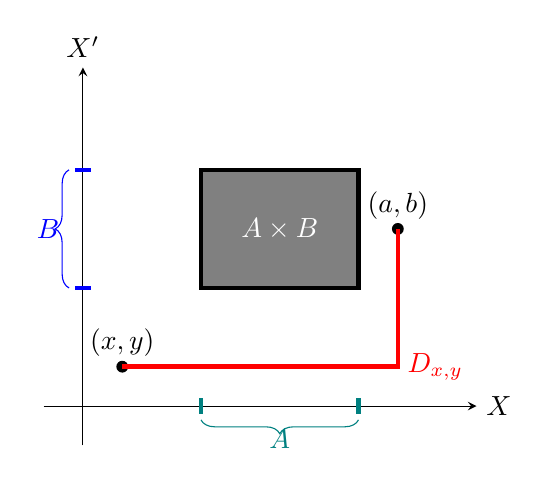
\begin{tikzpicture}
                \def\x{0.5}
                \def\y{0.5}
                \def\a{4}
                \def\b{2.25}
    
                % Ejes cartesianos
                \draw[-stealth] (-0.5, 0) -- (5, 0) node[right] {$X$};
                \draw[-stealth] (0, -0.5) -- (0, 4.3) node[above] {$X'$};
    
                % Marcas en el eje horizontal del conjunto A
                \draw[ultra thick, teal] (1.5,0.1) -- (1.5,-0.1);
                \draw[ultra thick, teal] (3.5,0.1) -- (3.5,-0.1);
                % Señalizacion A
                \draw[decorate,decoration={brace,amplitude=5pt,mirror}, teal, yshift=-5pt]
                (1.5,0) -- (3.5,0) node[midway,below] {$A$};
    
                % Marcas en el eje horizontal del conjunto B
                \draw[ultra thick, blue] (0.1,1.5) -- (-0.1,1.5);
                \draw[ultra thick, blue] (0.1,3) -- (-0.1,3);
                % Señalizacion B
                \draw[decorate,decoration={brace,amplitude=5pt}, blue, xshift=-5pt]
                (0,1.5) -- (0,3) node[midway,left] {$B$};
                
                % Conjunto AxB
                \draw[fill=gray, ultra thick] (1.5,1.5) rectangle (3.5,3);
                \node[white] at (2.5,2.25) {$A\times B$};
    
                % Punto (a,b)
                \fill (\a,\b) circle (0.075);
                \node[above] at (\a,\b) {$(a,b)$};
    
                % Punto (x,y)
                \fill (\x,\y) circle (0.075);
                \node[above] at (\x,\y) {$(x,y)$};
    
                % Conjunto D_{x,y}
                \draw[red, ultra thick] (\x,\y) -- (\a,\y) -- (\a,\b);
                \node[red, right] at (\a,\y) {$D_{x,y}$};
            \end{tikzpicture}
            \caption{$x\notin A, y\in B$.}
        \end{subfigure}
        \end{comment}
        \caption{Conjunto $D_{x,y}$ para distintos casos.}
    \end{figure}

    Sea $(x,y)\in (X \times X') \setminus (A \times B)$.
    \begin{enumerate}
        \item Supongamos $x\notin A$ (Caso \ref{fig:Rel3.11.a}).
        
        Entonces $\{x\}\times X'$ es conexo por ser 
        homeomorfo a $X'$, y $(x,y),(x,b)\in \{x\}\times X'$.
        Además, $X\times \{b\}$ es conexo por ser homeomorfo a $X$, y $(a,b),(x,b)\in X\times \{b\}$.
        Por tanto, sea $D_{x,y}=X\times \{b\} \cup \{x\}\times X'$.
        Tenemos que $D_{x,y}$ es conexo por ser unión de conexos con intersección
        no vacía $\left((x,b)\in X\times \{b\}\cap \{x\}\times X'\right)$.
        Además, como $x\notin A$, $b\notin B$, entonces $D_{x,y}\subset (X \times X') \setminus (A \times B)$.
        Además, como $(a,b), (x,y)\in D_{x,y}$, entonces $(x,y)\in D_{x,y}\subset C(a,b)$.

        \item Supongamos $x\in A$ (Caso \ref{fig:Rel3.11.b}).
        
        En este caso es similar, solo que $D_{x,y}=X\times \{y\} \cup \{a\}\times X'$.
    \end{enumerate}

    Notemos que, para que $D_{x,y}\subset (X \times X') \setminus (A \times B)$,
    es necesario que $(a,b)\in (X\setminus A) \times (X'\setminus B)$, no basta con
    que $(a,b)\in (X\times X') \setminus (A\times B)$.
\end{ejercicio}

\begin{ejercicio}
    Sea $X$ el conjunto de los puntos de $ \bb{R}^2 $ con alguna coordenada racional. Prueba que $X$ con la topología inducida es un subconjunto conexo.\\

    Sea $X=\{(x,y)\in \bb{R}^2 \mid x\in \bb{Q} \lor y\in \bb{Q}\}=(\bb{R}\times \bb{Q}) \cup (\bb{Q}\times \bb{R})$.
\end{ejercicio}

\begin{ejercicio}
    Prueba que no existen aplicaciones continuas e inyectivas de $\bb{R}^2$ en $\bb{R}$.

    Sea $f:\bb{R}^2\to \bb{R}$ continua e inyectiva. Tenemos que, como $f$ es continua y $\bb{R}^2$ es conexo, $f(\bb{R}^2)\subset \bb{R}$ es conexo, luego es un intervalo, supongamos de extremos
    $a$ y $b$, $a<b$, $a,b\in \bb{R}$, o $\pm \infty$.

    Sea ahora $c\in f(\bb{R}^2)$ tal que $a<c<b$, y como $f$ es inyectiva, consideremos su preimagen $f^{-1}(c)\in \bb{R}^2$, que es única.
    Sea entonces la restricción de $f$ a $\bb{R}^2\setminus \{f^{-1}(c)\}$,
    que es un homeomorfismo entre $\bb{R}^2\setminus \{f^{-1}(c)\}$ y $A\setminus \{c\}$. Como $\bb{R}^2\setminus \{f^{-1}(c)\}$ es homeomorfo a $\bb{R}^2\setminus \{0\}$, es conexo, por lo que
    $A\setminus \{c\}\subset \bb{R}$ es conexo pero no es un intervalo, ya que $a,b\in A\setminus \{c\}$ y $c\notin A\setminus \{c\}$, lo que es una contradicción.
\end{ejercicio}

\begin{ejercicio}
    Sea $(X, \T)$ un espacio topológico y $\{A_i\}_{i \in I}$ una partición por subconjuntos conexos y abiertos de $(X, \T)$. Entonces $\{A_i\}_{i \in I}$ es la familia de componentes conexas de $X$.\\

    Demostrado en la Proposición \ref{prop:ParticionConexosAbiertos}.
\end{ejercicio}



\begin{ejercicio}
    Sea $ X = \{a, b, c, d, e\} $ y $ \T = \{X, \emptyset, \{a\}, \{c, d\}, \{a, c, d\}, \{b, c, d, e\}\} $. Calcula las componentes conexas de $(X, \T)$.

    \begin{equation*}
        \left\{\{a\}, \{b, c, d, e\}\right\}
    \end{equation*}
    Dicho conjunto tenemos que es una partición de $X$ por subconjuntos conexos y abiertos, por lo que son las componentes conexas de $(X, \T)$.
\end{ejercicio}

\begin{ejercicio}
    Denotemos por $ C((a, b), r) $ la circunferencia en $ \bb{R}^2 $ con centro $(a, b)$ y radio $r$. Demuestra que ninguno de los siguientes espacios topológicos es homeomorfo a cualquier otro:
    \begin{enumerate}
        \item $X_1 = C((0, 0), 1) $
        \item $X_2 = C((-1, 0), 1) \cup C((1, 0), 1) $
        \item $X_3 = C((-1, 0), 1) \cup C((1, 0), 1) \cup C\left(\left(0, \sqrt{3}\right), 1\right) $
        \item $X_4 = C((-1, 0), 1) \cup C((1, 0), 1) \cup (\bb{R} \times \{1\}) $.
    \end{enumerate}
    \begin{figure}[H]
        \begin{subfigure}[c]{0.5\linewidth}
            \centering
            \begin{tikzpicture}
                % Ejes cartesianos
                \draw[-stealth, dashed] (-1.5, 0) -- (1.5, 0) node[right] {$x$};
                \draw[-stealth, dashed] (0, -1.5) -- (0, 1.5) node[above] {$y$};

                % Circunferencia
                \draw[teal] (0, 0) circle (1);

                % Marca el centro
                \fill (0,0) circle (0.075);
            \end{tikzpicture}
            \caption{$X_1 = C((0, 0), 1)$}
        \end{subfigure}\hfill
        \begin{subfigure}[c]{0.5\linewidth}
            \centering
            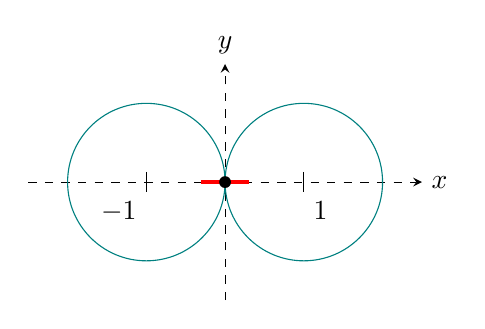
\begin{tikzpicture}
                % Ejes cartesianos
                \draw[-stealth, dashed] (-2.5, 0) -- (2.5, 0) node[right] {$x$};
                \draw[-stealth, dashed] (0, -1.5) -- (0, 1.5) node[above] {$y$};

                % Circunferencia
                \draw[teal] (-1, 0) circle (1);
                \draw[teal] (1, 0) circle (1);

                % Marca de punto de tangencia
                \draw[ultra thick, red] (-0.3,0) -- (0.3,0);
                \fill (0,0) circle (0.075);

                % Etiqueta en x=1, x=-1
                \draw (1,0.13) -- (1,-0.13) node[below right] {$1$};
                \draw (-1,0.13) -- (-1,-0.13) node[below left] {$-1$};
            \end{tikzpicture}
            \caption{$X_2 = C((-1, 0), 1) \cup C((1, 0), 1)$}
        \end{subfigure}\hfill
        \begin{subfigure}[c]{0.5\linewidth}
            \centering
            \begin{tikzpicture}
                % Ejes cartesianos
                \draw[-stealth, dashed] (-2.5, 0) -- (2.5, 0) node[right] {$x$};
                \draw[-stealth, dashed] (0, -1.7) -- (0, 3.3) node[above] {$y$};

                % Cálculo de raiz de 3
                \pgfmathsetmacro{\raiz}{sqrt(3)}
                
                % Centros de las circunferencias
                \coordinate (C1) at (-1, 0);
                \coordinate (C2) at (1, 0);
                \coordinate (C3) at (0, \raiz);
                % Circunferencia
                \draw[teal] (C1) circle (1);
                \draw[teal] (C2) circle (1);
                \draw[teal] (C3) circle (1);

                % Puntos de tangencia
                \coordinate (P1) at (-0.5, \raiz/2);
                \coordinate (P2) at (0.5, \raiz/2);
                \coordinate (P3) at (0, 0);

                % Marca de punto de tangencia
                \draw[ultra thick, red] ($(C1)!0.7!(P1)$) -- ($(C1)!1.3!(P1)$);
                \draw[ultra thick, red] ($(C2)!0.7!(P2)$) -- ($(C2)!1.3!(P2)$);
                \draw[ultra thick, red] ($(C1)!0.7!(P3)$) -- ($(C1)!1.3!(P3)$);
                \fill (P1) circle (0.075);
                \fill (P2) circle (0.075);
                \fill (P3) circle (0.075);

                % Etiqueta en x=1, x=-1
                \draw (1,0.13) -- (1,-0.13) node[below right] {$1$};
                \draw (-1,0.13) -- (-1,-0.13) node[below left] {$-1$};

                % Etiqueta en y=sqrt(3)
                \draw (0.13, \raiz) -- (-0.13, \raiz) node[left] {$\sqrt{3}$};
            \end{tikzpicture}
            \caption{\centering $X_3~=~C((-1, 0), 1) \cup C((1, 0), 1) \cup C\left(\left(0, \sqrt{3}\right), 1\right)$}
        \end{subfigure}
        \begin{subfigure}[c]{0.5\linewidth}
            \centering
            \begin{tikzpicture}
                % Ejes cartesianos
                \draw[-stealth, dashed] (-2.5, 0) -- (2.5, 0) node[right] {$x$};
                \draw[-stealth, dashed] (0, -1.5) -- (0, 1.5) node[above] {$y$};
                
                % Centros de las circunferencias
                \coordinate (C1) at (-1, 0);
                \coordinate (C2) at (1, 0);
                % Circunferencia
                \draw[teal] (C1) circle (1);
                \draw[teal] (C2) circle (1);

                \draw[teal] (-2.5, 1) -- (2.5, 1) node[right] {$y=1$};

                % Puntos de tangencia
                \coordinate (P1) at (-1,1);
                \coordinate (P2) at (1,1);
                \coordinate (P3) at (0,0);

                % Marca de punto de tangencia
                \draw[ultra thick, red] ($(C1)!0.7!(P1)$) -- ($(C1)!1.3!(P1)$);
                \draw[ultra thick, red] ($(C2)!0.7!(P2)$) -- ($(C2)!1.3!(P2)$);
                \draw[ultra thick, red] ($(C1)!0.7!(P3)$) -- ($(C1)!1.3!(P3)$);
                \fill (P1) circle (0.075);
                \fill (P2) circle (0.075);
                \fill (P3) circle (0.075);

                % Etiqueta en x=1, x=-1
                \draw (1,0.13) -- (1,-0.13) node[below right] {$1$};
                \draw (-1,0.13) -- (-1,-0.13) node[below left] {$-1$};
            \end{tikzpicture}
            \caption{\centering $X_4~=~C((-1, 0), 1) \cup C((1, 0), 1) \cup (\bb{R} \times \{1\}) $}
        \end{subfigure}
    \end{figure}

    Veamos en primer que toda circunferencia a la que se le quita un punto sigue siendo conexa. Tenemos que una circunferencia es homeomorfa a $\bb{S}^1$,
    que es conexo. Además, también tenemos que $\bb{S}^1\setminus \{p\}$ es conexo, y es homeomorfo a una circunferencia a la que se le quita un punto, 
    por lo que es conexo.

    No obstante, veamos que $\bb{S}^1\setminus \{p,q\}$ con $p\neq q$, es disconexo. Consideremos la recta $R=p+\cc{L}\left\{\vec{pq}\right\}$ que
    pasa por $p$ y $q$. Tenemos que $R$ divide $\bb{R}^2$ en dos semiplanos, ambos abiertos en $\T_u$, y al intersecar cada plano con $\bb{S}^1\setminus \{p,q\}$,
    obtenemos dos abiertos en $\T_{\bb{S}^1\setminus \{p,q\}}$ (los dos arcos de circunferencia que quedan) que son disjuntos y cuya unión es $\bb{S}^1\setminus \{p,q\}$,
    por lo que $\bb{S}^1\setminus \{p,q\}$ es disconexo.

    Veamos ahora que $X_1$ no es homeomorfo al resto. Supongamos que $f_i:X_1\to X_i$ es un homeomorfismo para $i=2,3,4$.
    Sean $p_i,q_i\in X_i$ tales que $p_i\neq q_i$ para $i=2,3,4$, no perteneciendo ambos a la misma circunferencia ni, en el caso de $X_4$, a la recta $y=1$.
    Entonces, $f_i^{-1}(p_i),f_i^{-1}(q_i)\in X_1$ son tales que $f_i^{-1}(p_i)\neq f_i^{-1}(q_i)$ por ser $f_i$ inyectiva.
    Consideremos ahora la restricción de $f_i$, ${f_i}_{\big| X_1\setminus \{f_i^{-1}(p_i), f_i^{-1}(q_i)\}}: X_1\setminus \{f_i^{-1}(p_i), f_i^{-1}(q_i)\} \to X_i\setminus \{p_i,q_i\}$,
    que es un homeomorfismo por ser $f_i$ homeomorfismo. Veamos ahira que $X_i\setminus \{p_i,q_i\}$ es disconexo para $i=2,3,4$.
    Como los puntos $p_i,q_i$ no pertenecen a la misma circunferencia, entonces todas las circunferencias son conexas. Además, como
    los puntos no son los puntos de tangencia, entonces $X_i\setminus \{p_i,q_i\}$ es la unión de conexos con intersección no vacía, por lo que son conexos.
    En concreto, para el caso de $X_4$, la recta es conexa por ser homeomorfa a $\bb{R}$ y, como los puntos que se han quitado no son de la recta, sigue siendo conexa.
    Por tanto, hemos visto que $X_i\setminus \{p_i,q_i\}$ es conexo, por lo que $X_1\setminus \{p_i,q_i\}$ es conexo, pero sabemos que no lo es por ser una circunferencia a la que se le han quitado dos puntos.
    Por tanto, llegamos a un absurdo, por lo que $X_1$ no es homeomorfo a $X_i$ para $i=2,3,4$.

    Veamos ahora que $X_2$ no es homeomorfo a $X_i$, con $i=3,4$. Supongamos que $f_i:X_2\to X_i$ es un homeomorfismo para $i=3,4$.
    Consideramos $p=(0,0)\in X_2$. Entonces, $X_2\setminus \{p\}$ es disconexo, ya que la recta $y=0$ divide $\bb{R}^2$ en dos semiplanos, ambos abiertos en $\T_u$,
    y al intersecar cada plano con $X_2\setminus \{p\}$, obtenemos dos abiertos en $\T_{X_2\setminus \{p\}}$ (las dos circunferencias a las que se le ha quitado el $(0,0)$)
    que son disjuntos y cuya unión es $X_2\setminus \{p\}$, por lo que $X_2\setminus \{p\}$ es disconexo. Sin embargo, $X_i\setminus \{f_i(p)\}$ es conexo para $i=3,4$,
    ya que sigue siendo unión de conexos con intersección no vacía (tienen más de un punto de tangencia).
    Por tanto, consideramos la restricción de $f_i$, ${f_i}_{\big| X_2\setminus \{p\}}: X_2\setminus \{p\} \to X_i\setminus \{f_i(p)\}$, que es un homeomorfismo por ser $f_i$ homeomorfismo.
    Como $X_2\setminus \{p\}$ es disconexo y $X_i\setminus \{f_i(p)\}$ es conexo, llegamos a un absurdo, por lo que $X_2$ no es homeomorfo a $X_i$ para $i=3,4$.

    Veamos ahora que $X_3$ no es homeomorfo a $X_4$. Supongamos que $f:X_3\to X_4$ es un homeomorfismo.
    Sea $p=(1,1)$, y como $f$ es un homeomorfismo, consideramos $f^{-1}(p)\in X_3$. Entonces, $X_3\setminus \{f^{-1}(p)\}$ es conexo,
    porque es la unión de conexos con intersección no vacía (tienen más de un punto de tangencia). Sin embargo, $X_4\setminus \{p\}$ es disconexo.
    Por tanto, consideramos la restricción de $f$, ${f}_{\big| X_3\setminus \{f^{-1}(p)\}}: X_3\setminus \{f^{-1}(p)\} \to X_4\setminus \{p\}$, que es un homeomorfismo por ser $f$ homeomorfismo.
    Como $X_3\setminus \{f^{-1}(p)\}$ es conexo y $X_4\setminus \{p\}$ es disconexo, llegamos a un absurdo, por lo que $X_3$ no es homeomorfo a $X_4$.
\end{ejercicio}

\begin{ejercicio}
Decide cuáles de los siguientes subespacios de $ \bb{R} $ y $ \bb{R}^2 $ son compactos. Razona la respuesta:
\begin{enumerate}
    \item $[0, \infty[$
    
    En todo este ejercicio, haremos uso del Corolario de Heine-Borel (Corolario \ref{coro:HeineBorel}), que afirma que los 
    compactos en $\bb{R}^n$ son los cerrados y acotados.

    En este caso, $[0,\infty[$ es cerrado pero no acotado, por lo que no es compacto.

    \item $A=[0, 1] \cap \mathbb{Q}$
    
    En este caso, $[0,1]\cap \mathbb{Q}$ es acotado, pero no sabemos si es cerrado. Veamos que existe una sucesión
    de elementos de $A$ que converge a un punto de $\bb{R}\setminus A$. Sea la sucesión $\{x_n\}_{n\in \bb{N}}$ definida por
    \begin{equation*}
        \left\{ \left( 1 + \frac{1}{n} \right)^n -2 \right\}_{n\in \bb{N}} \longrightarrow e-2
    \end{equation*}
    Dicha sucesión sabemos que es convergente, y converge a $e-2$.
    Tenemos que $x_n\in A$ para todo $n\in \bb{N}$, por lo que, por el Ejercicio \ref{ej:Sucesiones}.\ref{ej:Sucesiones.LimiteEnAdherencia},
    $e-2\in \ol{A}$. Como $e-2\notin \bb{Q}$, tenemos que $e-2\notin A$, por lo que $A\neq \ol{A}$ y, por tanto,
    $A$ no es cerrado. Por tanto, $A$ no es compacto.

    \item $A=\{(x, y) \in \bb{R}^2 \mid x \geq 1, 0 \leq y \leq \frac{1}{x}\}$.
    
    Tenemos que $A$ no está acotado, ya que $[1,+\infty[\times \{0\} \subset A$,
    y este no está acotado por no estarlo $[1,+\infty[$. Por tanto, $A$ no es compacto.

    \item $A=\{(x, y) \in \bb{R}^2 \mid |x| + |y| \leq 1\}$.
    
    En este caso, $A=\ol{B}_1(0,1)$ bola cerrada unidad para la norma 1.
    Por tanto, $A$ es cerrado y acotado, por lo que es compacto.

    \item $A=\bb{S}^1 \setminus \left\{\left(\frac{\sqrt{2}}{2}, -\frac{\sqrt{2}}{2}\right)\right\}$.
    
    Tenemos que $A$ es homeomorfo a $\bb{R}$, que no es compacto. Por tanto, $A$ no es compacto.

    \item $(]0, 1[, \T) $ donde $ \T = \{\emptyset, X\} \cup \{]0, 1 - \nicefrac{1}{n}[~\mid n \geq 2\}$.
    
    Sea $U_n=]0, 1 - \nicefrac{1}{n}[$. Tenemos que $U_n$ es abierto para todo $n\in \bb{N}$, y que $U_n\subset U_{n+1}$ para todo $n\in \bb{N}$.
    Veamos que $U_n$ es un recubrimiento por abiertos de $]0,1[$. Tenemos que:
    \begin{equation*}
        \bigcup_{n\in \bb{N}} U_n = \bigcup_{n\in \bb{N}} \left]0, 1 - \frac{1}{n}\right[
            = \lim_{n\to \infty} \left]0, 1 - \frac{1}{n}\right[ = ]0,1[
    \end{equation*}

    Supongamos ahora que existe un conjunto $I_0\subset \bb{N}$ finito tal que $\{U_n\}_{n\in I_0}$ es un subrecubrimiento de $]0,1[$.
    Sea $n_0=\max I_0$. Entonces,
    \begin{equation*}
        \bigcup_{n\in I_0} U_n = \bigcup_{n\in I_0} \left]0, 1 - \frac{1}{n}\right[ = \left]0, 1 - \frac{1}{n_0}\right[ \neq ]0,1[
    \end{equation*}
    donde la última igualdad se da porque $\nexists n\in \bb{N}$ tal que $\frac{1}{n}=0$, por lo que $1-\frac{1}{n_0}\neq 1$.

    Por tanto, $(]0,1[, \T)$ no es compacto.
    
    \item $(\bb{R}, \T) $ donde $ \T = \left\{O \subseteq \bb{R} \mid O = U \setminus B, U \in \T_u, B \subseteq \left\{\frac{1}{n} \mid n \in \bb{N}\right\}\right\}$
    
    Tomando $B=\emptyset$, vemos claramente que $\T_u\subset \T$. Sea $U_=]-n,n[\in \T_u\subset \T$ para $n\in \bb{N}$. Entonces, $\{U_n\}_{n\in \bb{N}}$ es un
    recubrimiento por abiertos de $\bb{R}$, ya que:
    \begin{equation*}
        \bigcup_{n\in \bb{N}} U_n = \bigcup_{n\in \bb{N}} ]-n,n[ = \bb{R}
    \end{equation*}

    Supongamos ahora que existe un conjunto $I_0\subset \bb{N}$ finito tal que $\{U_n\}_{n\in I_0}$ es un subrecubrimiento de $\bb{R}$.
    Sea $n_0=\max I_0$. Entonces,
    \begin{equation*}
        \bigcup_{n\in I_0} U_n = \bigcup_{n\in I_0} ]-n,n[ = ]-n_0,n_0[ \neq \bb{R}
    \end{equation*}

    Por tanto, $(\bb{R}, \T)$ no es compacto.
    
    \item La recta de Sorgenfrey.
    
    El razonamiento es análogo al caso anterior, ya que $\T_u\subset \T_S$. Por tanto, $(\bb{R}, \T_S)$ no es compacto.

    \item $\left(\mathbb{Q}, {\T_u}_{\big |\mathbb{Q}}\right)$.
    
    Es fácil ver que $\bb{Q}$ no es cerrado, ya que $\ol{Q}= \bb{R}\neq \bb{Q}$. Por tanto, $\bb{Q}$ no es cerrado, por lo que no es compacto.

    \item $X $ es un conjunto, $ p \in X $ un punto fijo y $ \T = \{O \subseteq X \mid p \in O\} \cup \{\emptyset\}$.
    
    Tenemos que $\T$ es la topología del punto incluido para $p$.
    
    Sabemos que si $X$ es finito, entonces $(X,\T)$ es compacto. Supongamos por tanto que $X$ es infinito. 
    Sea $U_x = \{x,p\}$ para $x\in X$. Entonces, $\{U_x\}_{x\in X}$ es claramente un recubrimiento por abiertos de $X$, ya que:
    \begin{equation*}
        X = \bigcup_{x\in X} \{x\} \subset \bigcup_{x\in X} \{x,p\} = \bigcup_{x\in X} U_x = X
    \end{equation*}

    Supongamos ahora que existe un conjunto $I_0\subset X$ finito tal que $\{U_x\}_{x\in I_0}$ es un subrecubrimiento de $X$. Es decir,
    \begin{equation*}
        X = \bigcup_{x\in I_0} U_x = \bigcup_{x\in I_0} \{x,p\} = I_0 \cup \{p\}
    \end{equation*}
    Como $I_0$ es finito, entonces $I_0\cup \{p\}$ es finito, por lo que $X$ es finito, lo que es una contradicción.

    Por tanto, tenemos que:
    \begin{equation*}
        \left(X, \T\right) \text{ es compacto} \sii X \text{ es finito}
    \end{equation*}

    \item $X $ es un conjunto, $ p \in X $ un punto fijo y $ \T = \{O \subseteq X \mid p \notin O\} \cup \{X\}$.
    
    Sea $\{U_i\}_{i\in I}$ un recubrimiento por abiertos de $X$, es decir, $U_i\in \T$ para todo $i\in I$ y:
    \begin{equation*}
        X = \bigcup_{i\in I} U_i
    \end{equation*}

    Tenemos $p\in X$, por lo que $\exists i_0\in I$ tal que $p\in U_{i_0}$. Entonces, $U_{i_0}\in \T$ y $p\in U_{i_0}$, por lo que $U_{i_0}=X$.
    Entonces $\{X\}$ es un subrecubrimiento de $X$ finito para cualquier recubrimiento de $X$, por lo que $X$ es compacto.

    \item $\bb{N} $ con la topología $ \T = \{\emptyset, \bb{N}\} \cup \{\{1, \ldots, n\} \mid n \in \bb{N}\} $.
    
    Sea $U_n=\{1,\ldots,n\}$ para $n\in \bb{N}$. Entonces, $\{U_n\}_{n\in \bb{N}}$ es un recubrimiento por abiertos de $\bb{N}$, ya que:
    \begin{equation*}
        \bb{N} = \bigcup_{n\in \bb{N}} \{1,\ldots,n\}
    \end{equation*}

    Tenemos que $U_n\subset U_{n+1}$ para todo $n\in \bb{N}$. Supongamos ahora que existe un conjunto $I_0\subset \bb{N}$ finito tal que $\{U_n\}_{n\in I_0}$ es un subrecubrimiento de $\bb{N}$.
    Sea $n_0=\max I_0$. Entonces,
    \begin{equation*}
        \bigcup_{n\in I_0} U_n = \bigcup_{n\in I_0} \{1,\ldots,n\} = \{1,\ldots,n_0\} \neq \bb{N}
    \end{equation*}
    ya que los naturales no tienen máximo.

\end{enumerate}
\end{ejercicio}

\begin{ejercicio}
    Sea $(X, \T)$ un espacio topológico. Prueba que si $ A, A' \subseteq X $ son subespacios compactos, entonces $ A \cup A' $ también es compacto.\\

    Demostrado en la Proposición \ref{prop:UnionCompactos}.
\end{ejercicio}


\begin{ejercicio}
    Sea $(X, \T)$ un espacio topológico Hausdorff. Prueba que si $\{A_i\}_{i \in I}$ son subespacios compactos de $X$, entonces $\bigcap\limits_{i \in I} A_i$ también es compacto.\\

    Demostrado en el Corolario \ref{coro:InterseccionCompactos}.
\end{ejercicio}

\begin{ejercicio}\label{ej:4.3.19}
    Sea $(X, \T)$ un espacio topológico compacto y supongamos que para cada $n \in \bb{N}$,
    $C_n$ es un subconjunto cerrado y no vacío tal que $C_{n+1} \subseteq C_n$. Prueba que $\bigcap\limits_{n\in \bb{N}} C_n \neq \emptyset$.\\

    Por reducción al absurdo, supongamos que $\bigcap\limits_{n\in \bb{N}} C_n = \emptyset$. Entonces, tenemos que $\{X\setminus C_n\}_{n\in \bb{N}}$ es un recubrimiento por abiertos de $X$, ya que:
    \begin{equation*}
        X = X\setminus \left(\bigcap\limits_{n\in \bb{N}} C_n\right) = \bigcup_{n\in \bb{N}} X\setminus C_n
    \end{equation*}
    donde he aplicado que $X\setminus \emptyset = X$. Como $X$ es compacto, entonces existe un subconjunto finito $I_0\subset \bb{N}$ tal que $\{X\setminus C_n\}_{n\in I_0}$ es un subrecubrimiento de $X$:
    \begin{equation*}
        X = \bigcup_{n\in I_0} X\setminus C_n = X\setminus \left(\bigcap_{n\in I_0} C_n\right)
    \end{equation*}
    Como $I_0$ es finito, sea $n_0=\max I_0$ y, como $C_{n+1}\subseteq C_n$ para todo $n\in \bb{N}$, entonces $C_{n_0} \subseteq C_n$ para todo $n\in I_0$, por lo que:
    \begin{equation*}
        X = \bigcup_{n\in I_0} X\setminus C_n = X\setminus \left(\bigcap_{n\in I_0} C_n\right) = X\setminus C_{n_0}
    \end{equation*}
    Por tanto, como $X=X\setminus C_{n_0}$, tenemos que $C_{n_0}=\emptyset$, lo que es una contradicción, ya que $C_{n_0}$ es no vacío. Por tanto, $\bigcap\limits_{n\in \bb{N}} C_n \neq \emptyset$.
\end{ejercicio}

\begin{ejercicio} \label{ej:4.3.20}
    Sea $(X, \T)$ un espacio Hausdorff y compacto y $f: X \to X$ una aplicación continua. Prueba que existe $A \subseteq X$ un subconjunto cerrado y no vacío tal que $f(A) = A$.\\

    Como $f$ es continua y va de un compacto a un Hausdorff, por el Teorema \ref{teo:ContinuaEntoncesCerrada}, tenemos que $f$ es cerrada. Vamos a definirnos la siguiente sucesión:
    \begin{equation*}
        C_1 = X \qquad C_{n+1} = f(C_n)
    \end{equation*}
    
    Aplicaremos el método de inducción para demostrar dos resultados. En primer lugar, veremos que $C_n$ es cerrado no vacío para todo $n\in \bb{N}$.
    \begin{itemize}
        \item \ul{Para $n=1$:}
        
        Como $C_1=X$, entonces $C_1$ es cerrado. Además, como $X\neq \emptyset$, entonces $C_1\neq \emptyset$.

        \item \ul{Supuesto cierto para $n$, veamos que se cumple para $n+1$:}
        
        Como $f$ es cerrada y $C_n$ es cerrado por hipótesis de inducción, entonces $C_{n+1}=f(C_n)$ es cerrado.
        Además, como $C_n\neq \emptyset$ por hipótesis de inducción, entonces por ser $f$ una aplicación, $C_{n+1}=f(C_n)\neq \emptyset$.
    \end{itemize}

    Veamos ahora que $C_{n+1}\subseteq C_n$ para todo $n\in \bb{N}$.
    \begin{itemize}
        \item \ul{Para $n=1$:}
        
        Como $f:X\to X$, tenemos que $f(X)\subset X$, por lo que: $$C_2=f(C_1)=f(X)\subset X=C_1$$

        \item \ul{Supuesto cierto para $n$, veamos que se cumple para $n+1$:}
        
        Como, por hipótesis de inducción, $C_{n+1}\subset C_n$ y $f$ es una aplicación, entonces $f(C_{n+1})\subset f(C_n)$. Por tanto,
        \begin{equation*}
            C_{n+2} = f(C_{n+1}) \subset f(C_n) = C_{n+1}
        \end{equation*}
    \end{itemize}

    Por el ejercicio anterior, el Ejercicio \ref{ej:4.3.19}, tenemos que $\bigcap\limits_{n\in \bb{N}} C_n \neq \emptyset$. Sea entonces $A=\bigcap\limits_{n\in \bb{N}} C_n\neq \emptyset$.
    Como la intersección arbitraria de cerrados es cerrada, tenemos que $A$ es cerrado. Veamos que $f(A)=A$.
    \begin{equation*}
        f\left(A\right)
        = f\left(\bigcap_{n\in \bb{N}} C_n\right)
        = \bigcap_{n\in \bb{N}} f\left(C_n\right)
        = \bigcap_{n\in \bb{N}} C_{n+1}
        = \bigcap_{n\in \bb{N}} C_n
        = A
    \end{equation*}

    Por tanto, $\exists A\subset X$ cerrado no vacío tal que $f(A)=A$.
\end{ejercicio}

\begin{ejercicio}[Teorema de la aplicación contractiva]
    Demuestra que si $X$ es un espacio métrico compacto y $f: X \to X$ es una aplicación contractiva (es decir, existe $K < 1$ tal que $d(f(x), f(y)) \leq K \cdot d(x, y)$ para todo $x, y \in X$),
    entonces existe un único punto $x \in X$ tal que $f(x) = x$.\\

    Como $f$ es contrativa, en particular es lipschitziana, y por el ejercicio \ref{ej:Tema2.1} es continua. Además, como $X$ es un espacio métrico, tenemos que es T2.
    Por tanto, por el ejercicio anterior, el Ejercicio \ref{ej:4.3.20}, tenemos que existe $A\subset X$ cerrado no vacío tal que $f(A)=A$.
    No obstante, en este ejercicio piden demostrar que $A$ tiene un único punto, y que este punto es el único punto fijo de $f$.\\

    Buscamos demostrar que $A$ es un conjunto unitario. Consideremos la aplicación:
    \Func{d}{X\times X}{\bb{R}}{(x,y)}{d(x,y)}
    función distancia de $X$ continua.
    Como $A\subset X$ es cerrado y $X$ es compacto, tenemos que $A$ es compacto, por lo que $A\times A$ es compacto. Por tanto, como $d$ es continua,
    $d(A\times A)\subset \bb{R}$ es compacto, y como $\bb{R}$ es un espacio métrico, tenemos que $d(A\times A)$ es cerrado y acotado,
    y en particular alcanza su máximo. Es decir,
    \begin{equation*}
        \exists x_0,y_0\in A \text{ tal que } d(x_0,y_0)\geq d(x,y)\quad \forall x,y\in A
    \end{equation*}

    Como $f(A)=A$, entonces $\exists x_1,y_1\in A$ tales que $f(x_1)=x_0$ y $f(y_1)=x_0$. Entonces, tenemos que:
    \begin{multline*}
        d(x_0,y_0) = d(f(x_1),f(y_1)) \leq K\cdot d(x_1,y_1) \leq K\cdot d(x_0,y_0)
        \Longrightarrow \\ \Longrightarrow (1-K)\cdot d(x_0,y_0) \leq 0
    \end{multline*}
    Como $1-k>0$ y $d(x_0,y_0)\geq 0$, entonces tenemos que $d(x_0,y_0)=0$, por lo que $x_0=y_0$. Por tanto,
    \begin{equation*}
        0 \geq d(x,y) \Longrightarrow d(x,y)=0 \Longrightarrow x=y \hspace{2cm} \forall x,y\in A
    \end{equation*}
    Por tanto, tenemos que $A$ es un conjunto unitario, es decir, $A=\{x_0\}$. Como $f(A)=A$, entonces $f(x_0)=x_0$,
    por lo que $x_0$ es un punto fijo de $f$.\\
    
    Veamos ahora la segunda parte de la demostración, probando que es el único punto fijo de $f$. Sea $x'\in X$ otro punto fijo de $f$.
    \begin{multline*}
        d(x_0,x') = d(f(x_0),f(x')) \leq K\cdot d(x_0,x')
        \Longrightarrow \\ \Longrightarrow
        (1-K)\cdot d(x_0,x') \leq 0 \Longrightarrow d(x_0,x') = 0 \Longrightarrow x_0=x'
    \end{multline*}
\end{ejercicio}

\begin{ejercicio}
    Sea $(X, \T)$ un espacio topológico Hausdorff y $\{K_n\}_{n \in \bb{N}}$ una
    sucesión de compactos no vacíos en $X$ tal que $K_{n+1} \subseteq K_n$ para todo $n \in \bb{N}$.
    Demuestra que $K = \bigcap\limits_{n \in \bb{N}} K_n \neq \emptyset$
    y que si $U \in \T$ tal que $K \subseteq U$, entonces existe $n_0 \in \bb{N}$ tal que $K_m \subseteq U$.\\

    Como $X$ es Hausdorff y $K_n\subset X$ es compacto para todo $n\in \bb{N}$, 
    tenemos que $K_n$ es cerrado para todo $n\in \bb{N}$. Además, 
    como $K_{n+1}\subset K_n$ para todo $n\in \bb{N}$, entonces $K_n\cap K_1=K_n$
    para todo $n\in \bb{N}$, por lo que $K_n$ es cerrado en $K_1$ para todo $n\in \bb{N}$.
    Aplicando el Ejercicio \ref{ej:4.3.19} con $X=K_1$ y $C_n=K_n$,
    tenemos que $K\neq \emptyset$.
    
    \begin{comment}
    por lo que $X\setminus K_n\in \T$ es abierto para todo $n\in \bb{N}$, y por tanto
    $K_1\setminus K_n = K_1 \cap (X\setminus K_n)\in \T_{K_1}$ es abierto en $K_1$ para todo $n\in \bb{N}$.\\
    
    Supongamos ahora $K=\emptyset$. Entonces, tenemos que $\{K_1\setminus K_n\}_{n\in \bb{N}}$
    es un recubrimiento de $K_1$ por abiertos de $K_1$, ya que: 
    \begin{equation*}
        K_1 = K_1\setminus K
        = K_1 \setminus \left(\bigcap_{n\in \bb{N}} K_n\right)
        = \bigcup_{n\in \bb{N}} K_1\setminus K_n
    \end{equation*}    
    
    Como $K_1$ es compacto, existe un subconjunto finito $I_0\subset \bb{N}$ tal que $\{K_1\setminus K_n\}_{n\in I_0}$ es un subrecubrimiento de $K_1$:
    \begin{equation*}
        K_1 = \bigcup_{n\in I_0} K_1\setminus K_n
        = K_1\setminus \left(\bigcap_{n\in I_0} K_n\right)
    \end{equation*}
    Como $I_0$ es finito, sea $n_0=\max I_0$ y, como $K_{n+1}\subset K_n$ para todo $n\in \bb{N}$, entonces
    $K_{n_0} \subset K_n$ para todo $n\in I_0$, por lo que:
    \begin{equation*}
        K_1 = \bigcup_{n\in I_0} K_1\setminus K_n
        = K_1 \setminus \left(\bigcap_{n\in I_0} K_n\right)
        = K_1 \setminus K_{n_0}
    \end{equation*}

    Por tanto, como $K_1\neq \emptyset$, tenemos que $K_{n_0}=\emptyset$, lo que es una contradicción, ya que $K_{n_0}$ es no vacío.
    Por tanto, $K\neq \emptyset$.

    \begin{observacion}
        Al empezar a hacer el ejercicio, se podría pensar que está demostrada esta primera parte en el Ejercicio \ref{ej:4.3.19}, pero no es así.
        En el Ejercicio \ref{ej:4.3.19} se pide que $(X,\T)$ sea compacto, mientras que en este ejercicio se pide que sea Hausdorff, entre otros cambios.
        Sí es cierto que la demostración es similar, aunque el papel de $X$ como compacto en dicho ejercicio es
        sustituido por el papel de $K_1$ como compacto en este ejercicio.
    \end{observacion}
    \end{comment}

    Supongamos ahora que $U\in \T$ tal que $K\subset U$. Entonces, $X \setminus U\in C_\T$, por lo que $K_1\setminus U\in C_{\T_{K_1}}$ es cerrado en $K_1$.
    Como $K_1$ es compacto, entonces $K_1\setminus U\subset K_1$ es compacto. Veamos que $\{K_1\setminus K_n\}_{n\in \bb{N}}$ es un recubrimiento de $K_1\setminus U$ por abiertos de $K_1$.
    \begin{equation*}
        K_1\setminus U \subset K_1\setminus K
        = K_1 \setminus \left(\bigcap_{n\in \bb{N}} K_n\right)
        = \bigcup_{n\in \bb{N}} K_1\setminus K_n
    \end{equation*}

    Como $K_1\setminus U$ es compacto, existe un subconjunto finito $I_0\subset \bb{N}$ tal que la familia $\{K_1\setminus K_n\}_{n\in I_0}$ es un subrecubrimiento de $K_1\setminus U$:
    \begin{equation*}
        K_1\setminus U \subset \bigcup_{n\in I_0} K_1\setminus K_n
        = K_1\setminus \left(\bigcap_{n\in I_0} K_n\right)
    \end{equation*}
    Como $I_0$ es finito, sea $n_0=\max I_0$ y, como $K_{n+1}\subset K_n$ para todo $n\in \bb{N}$, entonces
    $K_{n_0} \subset K_n$ para todo $n\in I_0$, por lo que:
    \begin{equation*}
        K_1\setminus U \subset \bigcup_{n\in I_0} K_1\setminus K_n
        = K_1\setminus \left(\bigcap_{n\in I_0} K_n\right)
        = K_1\setminus K_{n_0}
    \end{equation*}

    Por tanto, tenemos que $K_1\setminus U \subset K_1\setminus K_{n_0}$, por lo que $K_{n_0}\subset U$. Por tanto, $\exists n_0\in \bb{N}$ tal que $K_{n_0}\subset U$.


\end{ejercicio}

\begin{ejercicio}
    Encuentra contraejemplos de las afirmaciones siguientes:
    \begin{enumerate}
        \item En cualquier espacio métrico toda bola cerrada es un subespacio compacto.
        
        Las bolas cerradas son cerrados topológicos,  y son subconjuntos del espacio métrico. Si el espacio métrico es compacto, por la proposición \ref{prop:CerradoCompacto}, entonces las bolas cerradas son compactas.
        Por tanto, tenemos que buscar un espacio métrico que no sea compacto. Además, en el caso de $\bb{R}^n$, se ha visto que los compactos son los cerrados y acotados, por lo que tenemos que buscar un espacio métrico distinto.

        Por ejemplo, sea $(X,d_{disc})$ espacio métrico asociado a la la distancia discreta, con $X$ infinito. Además, sabemos que $X$ no es compacto, pues $(X,d_{disc})=(X,\T_{disc})$ y $X$ es infinito.
        Entonces, tenemos que:
        \begin{equation*}
            \ol{B}(0,1) = \{x\in X \mid d(x,0)\leq 1\} = X
        \end{equation*}
        Por tanto, como $X$ no es compacto, tenemos que $\ol{B}(0,1)$ no es compacto.

        \item En cualquier espacio métrico ninguna bola abierta puede ser un subespacio compacto.
        
        En todo espacio métrico, sabemos que compacto implica cerrado y acotado. Por tanto, hemos de encontrar una topología en la que una bola abierta sea cerrada.
        
        Por ejemplo, sea $(X,d_{disc})$ espacio métrico asociado a la la distancia discreta, $X$ finito. Como $X$ es finito, entonces $X$ es compacto. Entonces:
        \begin{equation*}
            B\left(0, 1\right) = \{x\in X \mid d(x,0)< 1\} = \{0\} \in C_{\T_{disc}}
        \end{equation*}
        Por tanto, como $X$ es compacto y $B(0,1)\in C_{\T_{disc}}$, tenemos que $B(0,1)$ es compacto.
    \end{enumerate}
\end{ejercicio}

\begin{ejercicio}
    Demuestra que no existe ninguna función continua \[f: \left([0, 1], {\T_u}_{\big| [0,1]}\right) \to (\bb{R}, \T_u)\] que verifique $f(x) \in \bb{R} \setminus \mathbb{Q}$ si $x \in \mathbb{Q}$ y $f(x) \in \mathbb{Q}$ si $x \in \bb{R} \setminus \mathbb{Q}$.
\end{ejercicio}

\begin{ejercicio}
    Sean $(X, \T)$ e $(Y, \mathcal{T'})$ espacios topológicos con $(X, \T)$ compacto. Prueba que la proyección $\pi_Y: X \times Y \to Y$ es cerrada.
\end{ejercicio}

\begin{ejercicio}
    Se dice que $C \subseteq \bb{R}^2$ es una curva de Jordan si $C = f([0, 1])$ para $f: [0, 1] \to \bb{R}^2$ una aplicación continua e inyectiva. Prueba que no existe una curva de Jordan que rellene el cuadrado $[0, 1] \times [0, 1]$.
\end{ejercicio}

\begin{ejercicio}
    Prueba que los subconjuntos compactos de la recta de Sorgenfrey son necesariamente numerables.
\end{ejercicio}